\subsection{Explicacion del modelo}
    La implementación del MapReduce para resolver el problema esta basado en el
    siguiente esquema:\\
    \begin{figure}[ht]
        \begin{adjustbox}{addcode={
            \begin{minipage}{\width}}{
                \caption{Esquema de un map reduce}
            \end{minipage}},rotate=360,center}
            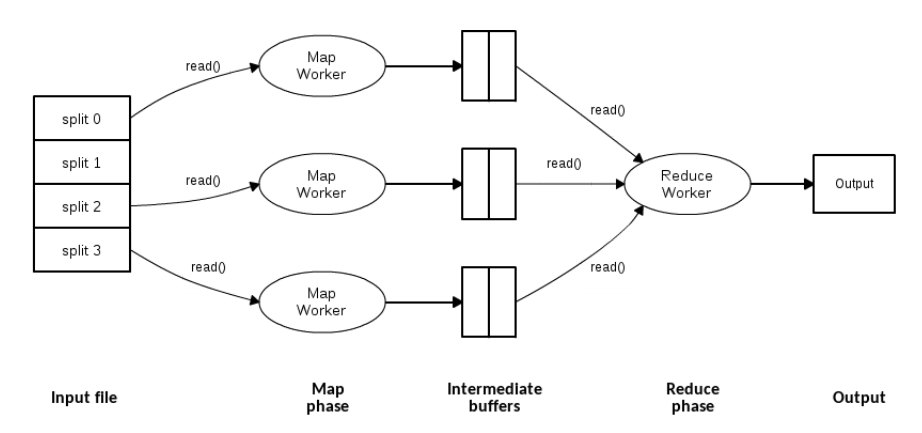
\includegraphics[scale=.6]{map_reduce_schema.png}
        \end{adjustbox}
    \end{figure}
    \FloatBarrier

    En nuestro caso creamos una clase llamada \code{MapReduce} la cual usa una
    libreria de \code{python} llamada \code{multiprocessing} en donde usamos el
    modulo \code{pool} el cual ofrece un medio conveniente para paralelizar la
    ejecución de una función a través de múltiples valores de entrada, distribuyendo
    los datos de entrada a través de procesos (paralelismo de datos).\\

    Entonces lo que hicimos fue instanciar dos \code{pool}, uno para hacer el map y
    el otro para el reduce de manera que el primero se le pasa como atributo la
    cantidad de worker en el cual se quiere paralelizar el problema y el segundo
    solo se usa uno de manera tal que la fase de reduce se la serie.

\subsection{Forma de ejecucion}
    Para ejecutar el calculo se debe ejecutar \lstinline[columns=fixed]{$ sh scripts/run.sh}.
    Este comando hace el calculo de multiplicacion de dos matrices.\\
    Para el caso de Amdahl multiplicamos dos matrices de 10x10
    con 1, 2, 4, 8, 16 y 32 threads.\\
    Para el caso de gustafson se usan siempre 4 threads multiplicando dos matrices
    de 2x2, 4x4, 8x8, 16x16, 32x32 y 64x64\\
    Luego para generar los graficos que vemos en el informe se debe
    ejecutar \lstinline[columns=fixed]{$ sh scripts/generate_output_data.sh}

\subsection{Datos sobre la computadora que se utilizó}
    El equipo sobre el que se realizarán las mediciones es una laptop con un
    procesador Intel core I7 que posee 4 nucleos a 2.7 Ghz, es decir, soporta
    hasta 4 threads en paralelo, con 16 Gb de memoria y corriendo sobre un
    sistema Linux.\\
    Para averiguar estos datos en linux se ejecutaron los siguientes comandos:\\
    \begin{itemize}
        \item Cantidad de cores: \lstinline[columns=fixed]{$ grep -c processor /proc/cpuinfo}
        \item Velocidad de reloj: \lstinline[columns=fixed]{$ lscpu | grep GHz}
        \item Memoria RAM: \lstinline[columns=fixed]{$ free -g}
    \end{itemize}